\chapter{Basic concepts} % Main chapter title
\label{chap:bc}

%----------------------------------------------------------------------------------------

\section{Introduction}
Why, and what does a system’s security consists of? Defining it is already an almost impossible task, because we would need to first understand what security is, which in itself is a very liable term.

Security properties are usually listed as follows:
\begin{itemize}
\item \textbf{Confidentiality}: ensuring that information is not accessible by unauthorized users;
\item \textbf{Integrity}: ensuring that information is not altered by unauthorized users in a way that is not detectable by the authorized ones;
\item \textbf{Authentication}: ensuring that authorized users actually are the people they claim to be.
\end{itemize}

This classification (often called CIA), however, is too simple and fallacious, because even if these are desirable properties for a secure system, they are not universally recognized and there are, in fact, many different versions of it.

%----------------------------------------------------------------------------------------

\section{Security vs. Safety}
We should never mistake security for safety, or vice versa:

\begin{itemize}
\item \textbf{Security}: quality of being secure, as in freedom from danger and/or from fear or anxiety of danger;
\item \textbf{Safety}: condition of being safe from undergoing or causing damage, injury or loss of any kind; in IT it is strongly connected to the concept of cyberphysical system (in turn closely related to the Internet of Things), because a non-secure system could negatively impact the physical safety of a user (e.g. in a smart factory a safe machine would be one that would stop its operations in a potentially dangerous situation).
\end{itemize}

%----------------------------------------------------------------------------------------

\section{Security costs}
Security has significant costs, for three fundamental reasons:

\begin{itemize}
\item the system is more \textbf{complex} (high redundancy);
\item implementation takes longer, and \textbf{maintenance} operations are needed more often than usual;
\item \textbf{workflow} is changed.
\end{itemize}

Before actually planning the system, we need to know what has to be made secure, why, and most importantly, against whom. We also need to remember that when security policies are too limiting (cumbersome, inefficient systems) or not understood (people need to know why they are required to do certain things in certain ways), users will always find a way to violate them, making them useless; this phenomenon is called \textbf{deimplementation}.

So, before we take any security measure, we must ask ourselves:

\begin{itemize}
\item \textbf{how much} does it cost?
\item how (much) are we \textbf{limiting} the users?
\item \textbf{what} are we protecting?
\item \textbf{why} are we protecting it?
\item \textbf{against whom} are we protecting it?
\end{itemize}

In other words, we must have understood clearly what is the operating context that we are working in.

%----------------------------------------------------------------------------------------

\section{Enterprise Architecture Framework}
An \textbf{enterprise architecture framework} (\textbf{EAF}) defines how to create and use an enterprise architecture. An architecture framework provides principles and practices for creating and using the architecture description of a system, dividing it into domains, layers or views, and offers models - typically matrices and diagrams - for documenting each view. This allows for making systemic design decisions on all the components of the system and making long-term decisions around new design requirements, sustainability, and support. It is a concept closely related to enterprise management, and any person, entity or business who wishes to work efficiently needs one.

There are many different EAF standards; among them we can find:

\begin{itemize}
\vspace{0.2em}
\item civil use frameworks (the most used):
\begin{itemize}
\item \textbf{COBIT}: framework for IT Governance and Control;
\item \textbf{TOGAF}: The Open Group Architecture Framework;
\end{itemize}
\vspace{0.2em}
\item military use frameworks:
\begin{itemize}
\item \textbf{DoDAF}: United States Department of Defense Architectural Framework;
\item \textbf{MODAF}: United Kingdom Ministry of Defense Architectural Framework;
\item \textbf{NAF}: NATO Architecture Framework;
\end{itemize}
\vspace{0.2em}
\item open-source frameworks:
\begin{itemize}
\item \textbf{SABSA}: a comprehensive framework for Enterprise Security Architecture and Service
Management; nowadays it is not used anymore because other EAFs have also incorporated security in their frameworks.
\end{itemize}
\end{itemize}

%-------------------------------------------

\subsection{EAF structure}

Almost all EAFs use \textbf{iterative} models, which better specify in each phase the concepts outlined in the previous ones. The first and most important phases of an EAF are the following:

\begin{itemize}
    \item \textbf{Preliminary Phase}: describes the first ideas for the enterprise, and defines its goals.
    \item \textbf{Architecture Vision}: better defines the framework by setting the scope, constraints and expectations for the project.
    \item \textbf{Business Architecture}: defines where the initial investments come from and how profit will be made (as well as how it will be used: EAFs are often used for non-profit organizations, too).
    \item \textbf{Requirements}: a recurrent phase among the most important ones, it ensures that every stage of a project is correctly executed and complies with any requirements that might exist. Requirements are mainly derived from the business architecture, and can either be 100\% satisfied or not satisfied at all (there is no in-between).
    \item \textbf{Information Systems Architecture}: defines the data needed in order for the enterprise to work properly; it does not specify network architectures, programs needed or other software assets, but instead assumes that data is the most valuable asset, and the one that security requirements will be defined on. Note that it is of the utmost importance to never, ever specify current technologies in security requirements, because they change too rapidly and even though they might become vulnerable in the future, the technical document will impose their use nonetheless. A note should be included saying that given a certain architecture, cryptography algorithms and security measures should be periodically revised and updated.
\end{itemize}

The remaining phases mostly describe the dynamic evolution of the enterprise, rather than security requirements.

\begin{figure}[H]
\centering
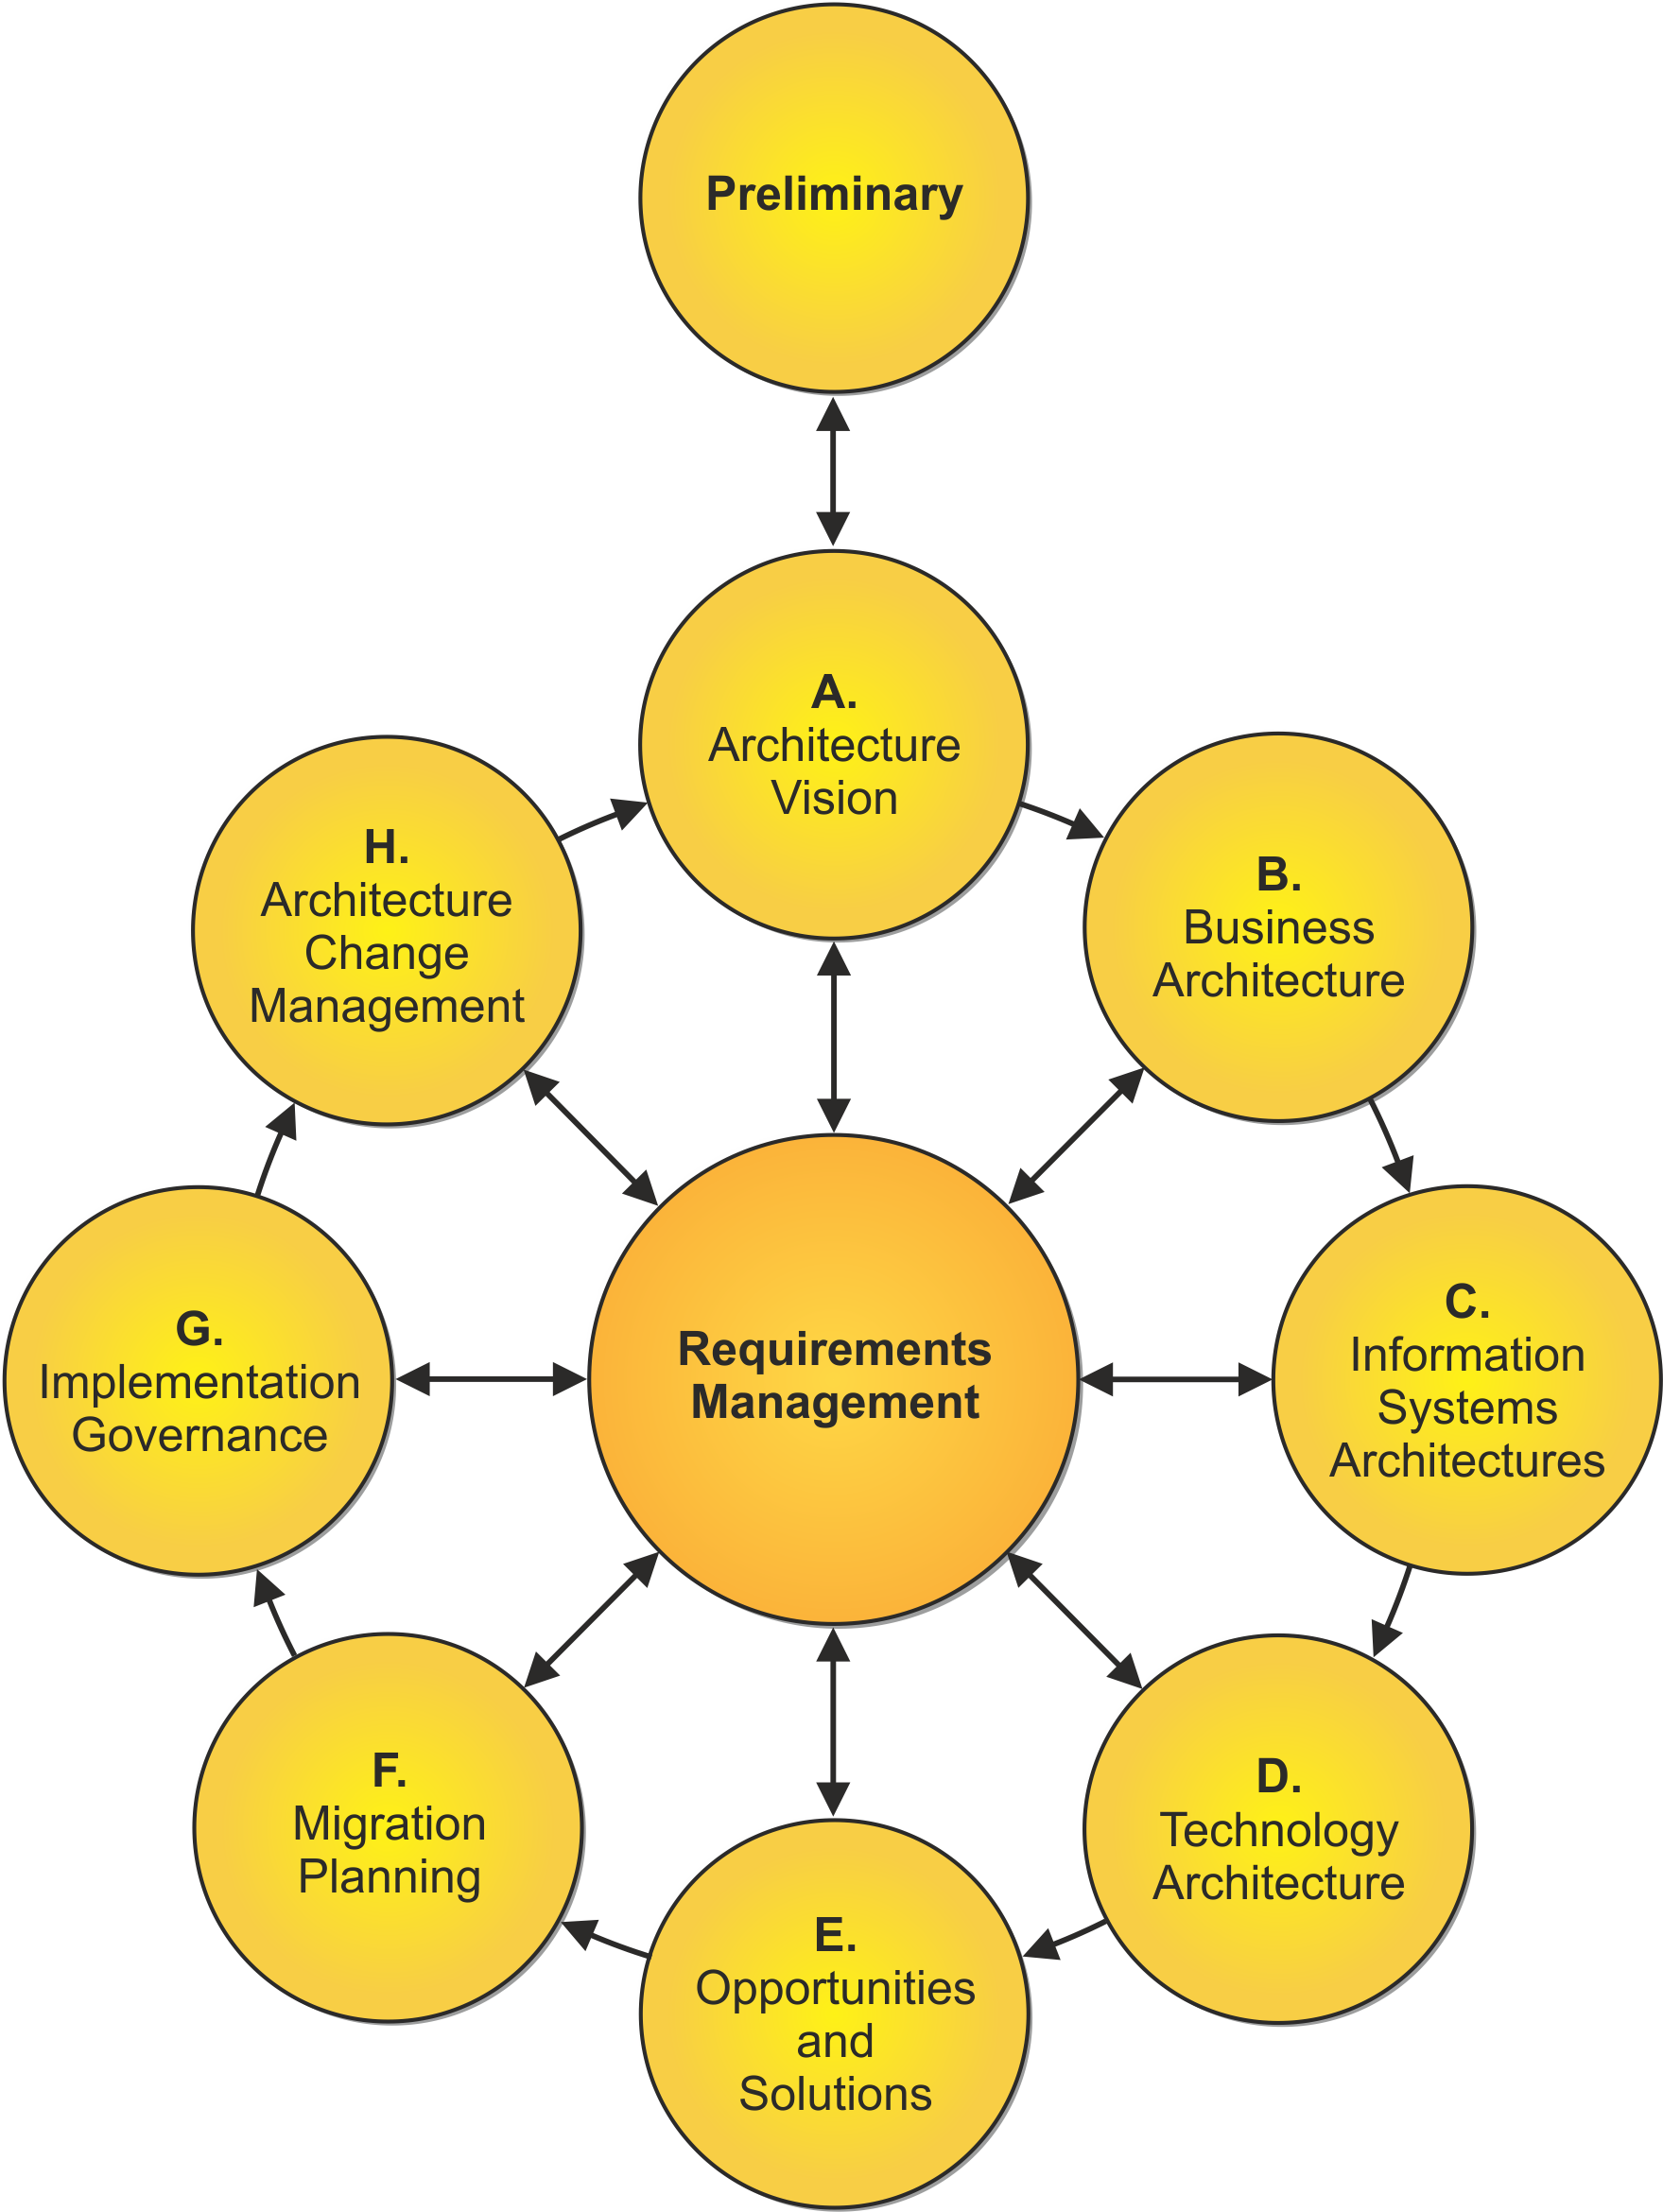
\includegraphics[scale=0.6]{img/togaf.png}
\decoRule
\caption{Example of an EAF structure (TOGAF).}
\label{fig:togaf}
\end{figure}

%-------------------------------------------

\subsection{Assets}
An \textbf{asset} is anything that represents a valuable resource for the enterprise. Protecting assets is the ultimate goal of security.

Assets usually fall into one of these categories:

\begin{itemize}
    \item \textbf{data} (typically the most valuable asset);
    \item \textbf{software components} (programs, applications, algorithms, etc.);
    \item \textbf{hardware components} (physical assets).
\end{itemize}

The security level of an asset derives from its properties; every asset has many, which can be set by the:

\begin{itemize}
    \item \textbf{law}: privacy laws, etc. (e.g. GDPR, National Security laws);
    \item \textbf{company}: whatever the company wants to do with its assets (e.g. guarantee to its users a certain level of privacy);
    \item \textbf{employer}: might be someone who needs extra security (e.g. the Department of Defense);
    \item \textbf{contract}: it could include Non Disclosure Agreements (NDAs) or other similar policies.
\end{itemize}

These properties, all of which are listed in the EAF, can either be \textbf{intrinsic} (imposed by an external entity, such as the law) or \textbf{extrinsic} (decided by the enterprise itself), and have to be specified in terms of \textbf{must}/\textbf{must not} (assets that 100\% have to comply to these properties) or \textbf{should}/\textbf{should not} (assets that must comply to these properties with at least a specified percentage).

All properties extend to all assets which handle other assets, e.g. if there is a requirement on the data, then all applications that handle it must comply to whatever requirements that data has. This means that security is as strong as the weakest link in the chain.

%----------------------------------------------------------------------------------------

\section{Risk management}
In general, we always need to have a plan in case something goes wrong. We do this by analyzing the working context in order to identify, evaluate and find countermeasures for all (or part of) possible risks:

\begin{enumerate}
    \item \textbf{risk identification};
    \item \textbf{risk evaluation};
    \item \textbf{implementation} of policies and countermeasures;
    \item \textbf{maintenance} of policies and countermeasures.
\end{enumerate}

Following these phases in order is mandatory, because points 3 and 4 are not possible without the first two.

%-------------------------------------------

\subsection{Risk assessment}
In order to evaluate risks we can use one of these two methodologies:

\begin{itemize}
    \item \textbf{qualitative risk assessment}: simple, clear and concise vision of risks;
    \item \textbf{quantitative risk assessment}: mathematical loss expectancy evaluation.
\end{itemize}

%----------------------

\subsubsection{Qualitative risk assessment}
Qualitative risk assessment uses a matrix to visually represent (in percentage) how much a risk is important. As seen in fig. \ref{fig:qualrisk}, the horizontal axis of the matrix indicates the risk's occurrence probability, while the vertical axis shows the risk's importance in terms of how much damage it would cause to the business (in either economical or reputational terms). This kind of evaluation offers a clear vision of what are the most serious risks, allowing us to identify those that should be patched as soon as possible.

\begin{figure}[H]
\centering
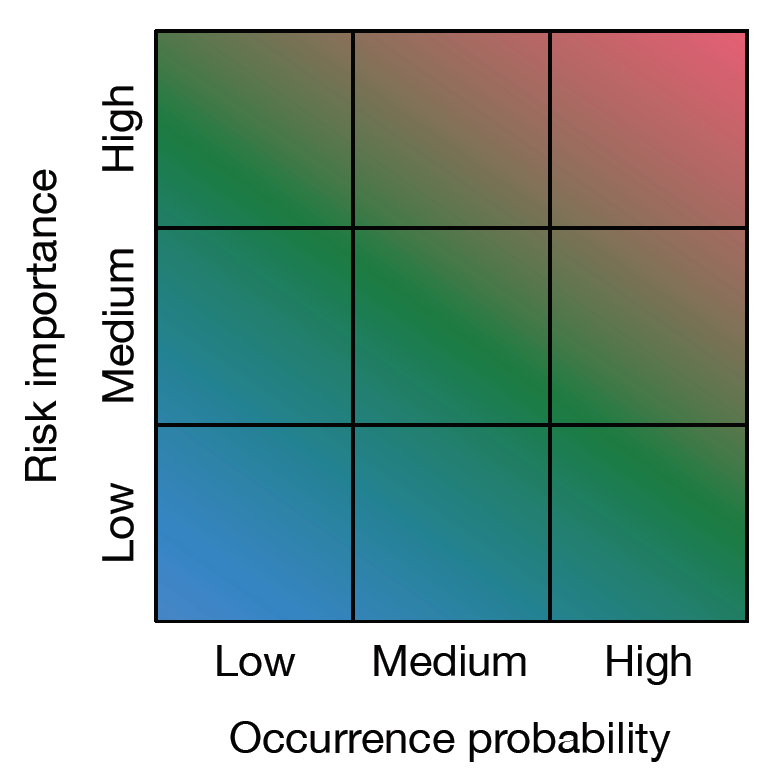
\includegraphics[scale=0.2]{img/qualitative_risk.png}
\decoRule
\caption{Qualitative risk assessment matrix.}
\label{fig:qualrisk}
\end{figure}

It must be noted, however, that not all risks should be covered; usually, risks in the central zone of the matrix (the one in green in fig. \ref{fig:qualrisk}) are considered acceptable, so they are acknowledged but nothing is done to avoid them.

Risks in the upper right area are mitigated in such a way that they can be moved to another zone: either towards the bottom to lower their occurrence probability, and/or the left, in order to lower their outcome (and possibly their cost, too); the exact direction depends on the cost and efficacy of the measures that need to be taken. This operation could be accomplished, for example, by transforming a primary asset into a secondary asset.

Generally, even though moving a risk directly to the lower left part of the matrix might seem ideal, doing this is not advised because the costs to achieve it would be too high, so it is usually better to deimplement some security measures and just keep the risks in the green area.

%----------------------

\subsubsection{Quantitative risk assessment}
Quantitative risk assessment is an analytical, less visual method that can be calculated using the following steps:

\begin{enumerate}
    \item \textbf{Asset Value (AV)} assignment: given an asset, we assign to it a certain economical value based on its importance;
    \item \textbf{Annual Rate of Occurrence (ARO) estimation}: as the name implies, we assess the number of times a certain risk is likely to occur in a year;
    \item \textbf{Exposure Factor (EF) estimation}: subjective, potential percentage of loss if a specific threat is realized;
    \item \textbf{Single-Loss Expectancy (SLE)}: $SLE = AV \cdot EF$; it represents the monetary value expected from the occurrence of a risk on an asset;
    \item \textbf{Annualized-Loss Expectancy (ALE)}: $ALE = SLE \cdot ARO$; as the formula implies, it is the product of the annual rate of occurrence (ARO) and the single loss expectancy (SLE).
\end{enumerate}

\emph{Beware of the average}: using it without knowing its probability distribution might be dangerous and counterproductive. It is usually safer and more informative to consider minimum and maximum values of a number.

%-------------------------------------------

\subsection{Risk analysis}

Correctly analyzing a risk requires many different phases and aspects to be taken in consideration, as illustrated in fig. \ref{fig:riskmodel}.

\begin{figure}[H]
\centering
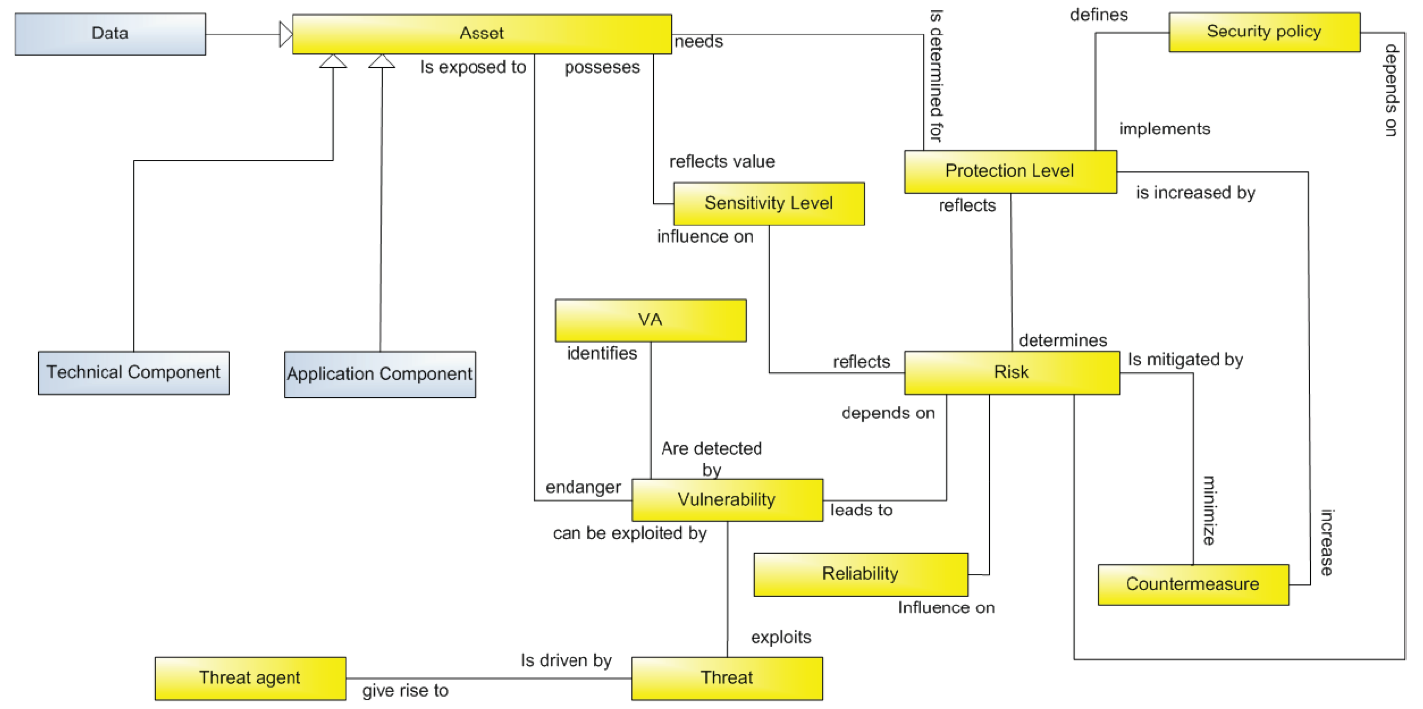
\includegraphics[scale=0.33]{img/risk_analysis.png}
\decoRule
\caption{A common risk analysis model.}
\label{fig:riskmodel}
\end{figure}

Given an \textbf{asset} and its \textbf{data}, the \textbf{sensitivity level} indicates how much the asset is important for the business; the higher this value, the higher the level of protection needed for the asset (and thus the lower the risk).

The \textbf{protection level} of an asset is directly correlated to its sensitivity level; it is implemented through:

\begin{enumerate}
    \item \textbf{security policies}: they mitigate the risk's occurrence (e.g. a database could implement an access control list, so that only authorized users could access it);
    \item \textbf{countermeasures}: they mitigate the risk's consequences \textit{after} its occurrence (e.g. a periodical system backup).
\end{enumerate}

A \textbf{risk} therefore depends on two large families of problems: \textbf{reliability}, which comprises all those factors that are determined by natural failures of the system, and \textbf{vulnerability}, the possibility that the system might be attacked by someone. Vulnerabilities are triggered by the existence of a bug in the protocols, components or the software used by the asset, namely in the:

\begin{itemize}
    \item \textbf{technical components} (hardware), usually subject to reliability problems;
    \item \textbf{application components} (software), usually subject to vulnerability problems.
\end{itemize}

Vulnerabilities can be found through the \textbf{Vulnerability Analysis} or \textbf{Vulnerability Assessment (VA)} process. It is a critical, open problem in software and network engineering, because even though some vulnerabilities are known and can be patched or at least partially covered, more often that not they are not known, so no countermeasures can be taken against them nor can they be taken into account when calculating risks. Thus, all vulnerabilities represent a serious \textbf{threat} that could be exploited by a \textbf{threat agent} - even though their existence only means that they have the potential to be abused of by a malicious agent, not that this will actually happen. In any case, a threat model can be used to better assess how a threat agent could damage an asset.

%----------------------------------------------------------------------------------------

\section{Threat model}
A \textbf{threat model} describes the capabilities that an attacker is assumed to be able to deploy against an asset. It should contain information about the resources available to the attacker, in terms of \textbf{available information}, \textbf{computing capability} (computational power depends on the attack) and \textbf{control of the system} (what the attacker would be able to do). The model also specifies the attacker's goals and how serious this person would be about his or her actions.

The threat model is necessary to define the risk probability, and it depends on the asset and the attacker's goals: the higher the goals, the greater the attacker's capabilities. Obviously, the model does not discuss physical threats only; many assets are immaterial, such as industrial secrets, and once they fall into the hands of an attacker they can be considered forever lost - even if the business still possesses them.

%-------------------------------------------

\subsection{Internet threat model}
\label{sec:internet_threat_model}
The generic Internet threat model (the one that is mostly used for devices connected to the Internet \textit{and} by people with a speck of brain) assumes these four points:

\begin{itemize}
    \item \textbf{Kerckhoff's principle}: the attacker knows everything about the system under attack. \textit{Security by obscurity}, an ideal which aims to make a system secure by intentionally hiding as many details about it as possible, should \textit{never} be pursued;
    \item the attacker has \textbf{enough computational power}: it might not always be limited to off-the-shelf\footnote{The definition of "off-the-shelf" actually depends on the level of the threat that we are talking about. An example: WiMax chipsets are nowhere to be found nowadays, because it is a dead standard; in order to get one to hack AeroMax communications at an airport, an attacker must either be a regular customer of AeroMax chipsets (which is extremely unlikely), or have a software defined radio and have developed the WiMax standard. Hacking AeroMax communications thus \textit{is} possible, but it actually costs too much for a single attacker to represent a real threat.} systems, as some attackers could also use highly specialized devices or tools, like AWS (Amazon Web Services);
    \item the attacker has \textbf{control of communication systems}: the attacker could inject data in the network. Note that the attacker might not be in full control the network, and/or could need to hide its presence, so it could either be able to only send data (active attacks, blind or almost blind) or to receive only (passive attacks);
    \item \textbf{does not} have control of the endpoints (these systems are protected).
\end{itemize}

In other words, even if the systems are not yet violated, the communication system might be
insecure. This assumption, however, can be relaxed in some cases.

%----------------------

\subsubsection{Attack examples}
\begin{itemize}

    \vspace{0.2em}
    
        \item \textbf{Passive attacks}
        \begin{itemize}
            \item Confidentiality violations
            \item Password stealing
            \item Offline cryptographic attacks
        \end{itemize}
        
    \vspace{0.2em}
        
    \item \textbf{Active attacks} (blind attacks)
        \begin{itemize}
            \item Replay attacks (a valid data transmission is maliciously or fraudulently repeated or delayed)
            \item Message insertion
            \item Message deletion
            \item Message modification
        \end{itemize}
\end{itemize}

These two kinds of attacks are very different in nature. A passive attacker usually has a very privileged position in the network, and his/her sending something in it would probably highlight his/her presence. For this reason, he/she usually just stays silent and only receives data.

%-------------------------------------------

\subsection{Network topology}
We cannot talk about threats without knowing the topology of the network we are working with, because it allows us to understand what an attacker is capable of as well as what he/she might desire to do, and how the network itself can be protected.

Depending on the topology, an attack can be classified as:

\begin{itemize}
    \item \textbf{on-path}: the attacker is on the \textit{natural} path of the data between the endpoints, either by sheer luck or thanks to his/her capabilities;
    \item \textbf{off-path}: the attacker does not see the data naturally flowing from a point A to another point B; in order to avoid being detected, he/she will have to pretend being B, but will not be able to see B's replies to A (blind attack);
    \item \textbf{link-local}: this is the worst case scenario, since the attacker is on the same link of the endpoint, in the same subnet or physically attached to the same switch/access point, a privileged position which permits a vast number of attacks.
\end{itemize}

We can assume that the attacker is off-path if and only if we control every single router and link between points A and B, and can be sure that the attacker has not violated any of these devices. Is this really feasible?

The answer to this question is that it depends on the geographical routing of the data, which in turn depends on the big communication links between the source and destination.

For example, there was once a project to lay a fiber optic cable between America and Asia, with one of the main exchange points in Hong Kong; the USA asked for this point to be removed, in order to avoid China's control, as they would have enabled on-path attacks. This request has not been satisfied, and thus the project has never been completed.

Note that mistakes in the routing tables that send data through places that should not be receiving them (e.g. San Francisco-Seattle through China) are at the order of the day, so in conclusion, never, ever assume that the attack is off-path, because an attacker can become on-path through a secondary attack to the routing.